%%%%%%%%%%%%%%%%%%%%%%%%%%%%%%%%%%%%%%%%%
% FRI Data Science_report LaTeX Template
% Version 1.0 (28/1/2020)
%
% Jure Demšar (jure.demsar@fri.uni-lj.si)
%
% Based on MicromouseSymp article template by:
% Mathias Legrand (legrand.mathias@gmail.com)
% With extensive modifications by:
% Antonio Valente (antonio.luis.valente@gmail.com)
%
% License:
% CC BY-NC-SA 3.0 (http://creativecommons.org/licenses/by-nc-sa/3.0/)
%
%%%%%%%%%%%%%%%%%%%%%%%%%%%%%%%%%%%%%%%%%


%----------------------------------------------------------------------------------------
%	PACKAGES AND OTHER DOCUMENT CONFIGURATIONS
%----------------------------------------------------------------------------------------
\documentclass[fleqn,moreauthors,10pt]{ds_report}
\usepackage[english]{babel}

\graphicspath{{fig/}}




%----------------------------------------------------------------------------------------
%	ARTICLE INFORMATION
%----------------------------------------------------------------------------------------

% Header
\JournalInfo{UL FRI - Biomedical signal and image processing}

% Type of report
\Archive{Assigment 1 Report}

% Article title
\PaperTitle{Detecting heart beats (QRS complex detection)}

% Authors and their info
\Authors{Aljaz Mur Erzen\textsuperscript{1}}
\affiliation{\textsuperscript{1}\textit{ae4664@student.uni-lj.si, 63160011}}

% Keywords
\Keywords{hearbeat, detection, signal}
\newcommand{\keywordname}{Keywords}


%----------------------------------------------------------------------------------------
%	ABSTRACT
%----------------------------------------------------------------------------------------

%----------------------------------------------------------------------------------------

\begin{document}

% Makes all text pages the same height
\flushbottom

% Print the title and abstract box
\maketitle

% Removes page numbering from the first page
\thispagestyle{empty}

%----------------------------------------------------------------------------------------
%	ARTICLE CONTENTS
%----------------------------------------------------------------------------------------

\section*{Introduction}
	
Automatic heartbeat detection plays a key role in analyzing streams of recorded ECG signals, finding abnormalities and predicting possible heart diseases. Due to significance of the implications, there is a lot of motivation to improve performance of existing detection algorithms.

This report describes how we implemented and modified detection algorithm described by the original article \cite{ding}.

%------------------------------------------------

\section*{Article interpretation}

The detector described in original article focuses on efficiency while maintaining sensitivity and positive prediction metrics of competing algorithms. The important part of its design is \textit{candidate sifting} based on simple thresholds to reduce number of samples that need to be analyzed as a possible R-peak candidates. This is done by two stages of threshold sifting and a final variation ratio test. 

\begin{figure}[ht]\centering
	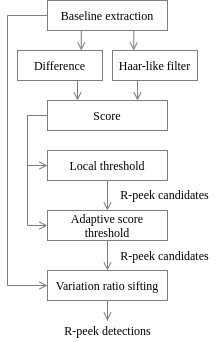
\includegraphics[width=0.6\linewidth]{ding-detector-diagram.png}
	\caption{\textbf{Diagram of the detector algorithm.} First we calculate a scoring function for every sample in the signal and then apply three stages of R-peak candidate sifting.}
	\label{fig:diagram}
\end{figure}

Descriptions of some parts of the detection algorithm are vague or even contain some mistakes. This section will cover how we interpreted those sections of the algorithm. It is advised to study the original article first.

\subsection*{Haar-like matching filter}

To find peaks, we could apply Laplacian of a Gaussian or take some other approach mimicking derivate of a signal. The article proposes using second degree difference of sequential points and a Haar-like matching filter. Both of them do not require Fourier transform and can easily be computed as a FIR filters.

\begin{figure}[!ht]\centering
	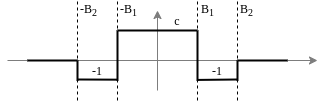
\includegraphics[width=0.8\linewidth]{haar-like.png}
	\caption{\textbf{Unit response of Haar-like matching filter.} The output of the filter is equal as a convolution of the input with the plotted signal.}
	\label{fig:haar-like}
\end{figure}

Description of FIR filter from the original article contained indexing mistake, but described the process in enough detail to be corrected. Given input signal $x(n)$ and parameters $B_1$ and $B_2$, we computed output of the filter $y(n)$ using following equations:

\begin{equation}
	\begin{aligned}
		y_1(n) & = y_1(n-1) + x(n+B_1) - x(n-B_1-1) \\
		y_2(n) & = y_2(n-1) + x(n+B_2) - x(n-B_2-1) \\
		y(n) & = -y_2(n) + (c+1)*y_1(n)
	\end{aligned}
\end{equation}

As advised in the original article, we selected $B_1 = 7$ and $B_2 = 15$ for testing on signal with sampling frequency $F_s = 250$.

Unfortunately, this FIR notation cannot be easily translated into Matlab, because parts $x(n+B_1)$ and $x(n+B_2)$. This is why we re-parametrized the first equation with $n \mapsto n - B_1$ and introduced translated $y_1$ as $u_1(n) = y_1(n - B_1)$. This can be done due to convolution's translation invariance. Resulting form is now $u_1(n) = u_1(n-1) + x(n) - x(n-2B_1-1)$ and 
can now make use of Matlab's \texttt{filter} function as with parameters \texttt{a=[1 1]} and \texttt{b=[1; zeros(2*B1-1); -1]}. To get $y_1$, we only have to apply reverse translation.

Similar was done for $y_2$. This improvement significantly decreased execution time in comparison with for loop implementation.

\subsection*{Adaptive score threshold}

After the first sifting of the R peak candidates, we perform \textit{adaptive score threshold}. It is adapted to global score magnitude and local regularity of the previous detected heartbeats. For a peak candidate $n$, following must be true: 
\begin{equation}
	abs(score(n)) > W_1 W_2
\end{equation}
Where $W_1$ is factor adapting to local peak amplitude and $W_2$ thresholds the peak regularity. This section leaves out information about setting quite a few of the parameter settings. We observed best results with $T = 1000$, $\beta_1 = 0.1$, $\beta_2 = 0.1$, $\tau_1 = \frac{6}{16}$, $\tau_2 = \frac{4}{16}$, $\tau_3 = \frac{3}{16}$, $\tau_4 = \frac{2}{16}$, $\tau_5 = \frac{1}{16}$.

These parameters were found by manual testing and adjustment. Almost surely, there are better configurations, but because current implementation of the algorithm has large startup and shutdown overhead, the parameter testing process is time intensive.

\section*{Implementation and testing}

Algorithm was implemented in Matlab programming language and used Bash scripts and Physionet's WFDB toolkit \cite{wfdb} for preparing, converting input data and evaluating detector output. The algorithm was developed and tested on data from LTST database \cite{ltst} containing 86 records each containing 2 or 3 ECG signals with mean duration 23.1h (std = 3.03h).

On a desktop computer with processor Processor AMD Ryzen 5 1600 Six-Core and Matlab version 9.9.0, mean running time of the detector analyzing one of the records was 118.11s (std = 25.93s).

\section*{Results}

The implementation of the algorithm achieved following results:

\begin{table}[hbt]
	\caption{Results of our implementation compared with results from the original article.}
	\centering
	\begin{tabular}{l | r r}
		\toprule
		                    & Our & Original article \\
		\midrule
		Beats				        & $8.863.647$ & $109.494$ \\
		False negatives     & $42030$			& $73$ \\
		False positives	    & $150283$		& $134$ \\
		Sensitivity 		    & $99.526\%$  & $99.933\%$ \\
		Positive prediction & $98.325\%$  & $99.878\%$ \\
		\bottomrule
	\end{tabular}
	\label{tab:label}
\end{table}

\section*{Discussion}

As a proof-of-concept implementation, the results are relatively good, compared with state-of-the-art algorithms discussed in original article. The comparison to the original article may not be appropriate due to different testing datasets and their sizes.

During the testing of the algorithm we have encountered some cases of false positive or and false negatives that were a consequence of baseline extraction. Because we used a IIR filter for baseline extraction, its non-linear phase shift properties distorts the heartbeat to become unrecognizable even to the human eye. To address this, we could use some other method for baseline extraction, maybe even local low-degree polynomial regression to predict the baseline using RANSAC.

The main pitfall of the implementation are parameter settings, which could be greatly improved by automated parameter testing. This would require rework of the testing framework and maybe even a rewrite of the algorithm to a more efficient programming language. 

\bibliographystyle{unsrt}
\bibliography{report}


\end{document}
